
\documentclass[letterpaper,hide notes,xcolor={table,svgnames},10pt]{beamer}
\def\showexamples{t}


%\usepackage[svgnames]{xcolor}

%% Demo talk
%\documentclass[letterpaper,notes=show]{beamer}

\usecolortheme{crane}
\setbeamertemplate{navigation symbols}{}

\usetheme{MyPittsburgh}
%\usetheme{Frankfurt}

%\usepackage{tipa}

\usepackage{hyperref}
\usepackage{graphicx,xspace}
\usepackage[normalem]{ulem}
\usepackage{multicol}
\usepackage{amsmath,amssymb,amsthm,graphicx,xspace}
\newcommand\SF[1]{$\bigstar$\footnote{SF: #1}}

\usepackage[default]{sourcesanspro}
\usepackage[T1]{fontenc}
\usepackage[scaled]{beramono}
\usepackage{tikzpagenodes}

\newcounter{tmpnumSlide}
\newcounter{tmpnumNote}


% old question code
%\newcommand\question[1]{{$\bigstar$ \small \onlySlide{2}{#1}}}
% \newcommand\nquestion[1]{\ifdefined \presentationonly \textcircled{?} \fi \note{\par{\Large \textbf{?}} #1}}
% \newcommand\nanswer[1]{\note{\par{\Large \textbf{A}} #1}}


 \newcommand\mnote[1]{%
   \addtocounter{tmpnumSlide}{1}
   \ifdefined\showcues {~\tiny\fbox{\arabic{tmpnumSlide}}}\fi
   \note{\setlength{\parskip}{1ex}\addtocounter{tmpnumNote}{1}\textbf{\Large \arabic{tmpnumNote}:} {#1\par}}}

\newcommand\mmnote[1]{\note{\setlength{\parskip}{1ex}#1\par}}

%\newcommand\mnote[2][]{\ifdefined\handoutwithnotes {~\tiny\fbox{#1}}\fi
% \note{\setlength{\parskip}{1ex}\textbf{\Large #1:} #2\par}}

%\newcommand\mnote[2][]{{\tiny\fbox{#1}} \note{\setlength{\parskip}{1ex}\textbf{\Large #1:} #2\par}}

\newcommand\mquestion[2]{{~\color{red}\fbox{?}}\note{\setlength{\parskip}{1ex}\par{\Large \textbf{?}} #1} \note{\setlength{\parskip}{1ex}\par{\Large \textbf{A}} #2\par}\ifdefined \presentationonly \pause \fi}

\newcommand\blackboard[1]{%
\ifdefined   \showblackboard
  {#1}
  \else {\begin{center} \fbox{\colorbox{blue!30}{%
         \begin{minipage}{.95\linewidth}%
           \hspace{\stretch{1}} Some space intentionally left blank; done at the blackboard.%
         \end{minipage}}}\end{center}}%
         \fi%
}

\newcommand{\Rplus}{\protect\hspace{-.1em}\protect\raisebox{.35ex}{\small{\small\textbf{+}}}}
\newcommand{\CPP}{\mbox{C\Rplus\Rplus}\xspace}

%\newcommand\q{\tikz \node[thick,color=black,shape=circle]{?};}
%\newcommand\q{\ifdefined \presentationonly \textcircled{?} \fi}

\usepackage{listings,listings-rust}
\lstset{basicstyle=\footnotesize\ttfamily,
	breaklines=true,
	aboveskip=15pt,
  	belowskip=15pt,
	frame=lines,
	numbers=left, basicstyle=\scriptsize, numberstyle=\tiny, stepnumber=0, numbersep=2pt
}

\usepackage{siunitx}
\newcommand\sius[1]{\num[group-separator = {,}]{#1}\si{\micro\second}}
\newcommand\sims[1]{\num[group-separator = {,}]{#1}\si{\milli\second}}
\newcommand\sins[1]{\num[group-separator = {,}]{#1}\si{\nano\second}}
\sisetup{group-separator = {,}, group-digits = true}

%% -------------------- tikz --------------------
\usepackage{tikz}
\usetikzlibrary{positioning}
\usetikzlibrary{arrows,backgrounds,automata,decorations.shapes,decorations.pathmorphing,decorations.markings,decorations.text,decorations.pathreplacing}

\tikzstyle{place}=[circle,draw=blue!50,fill=blue!20,thick, inner sep=0pt,minimum size=6mm]
\tikzstyle{transition}=[rectangle,draw=black!50,fill=black!20,thick, inner sep=0pt,minimum size=4mm]

\tikzstyle{block}=[rectangle,draw=black, thick, inner sep=5pt]
\tikzstyle{bullet}=[circle,draw=black, fill=black, thin, inner sep=2pt]

\tikzstyle{pre}=[<-,shorten <=1pt,>=stealth',semithick]
\tikzstyle{post}=[->,shorten >=1pt,>=stealth',semithick]
\tikzstyle{bi}=[<->,shorten >=1pt,shorten <=1pt, >=stealth',semithick]

\tikzstyle{mut}=[-,>=stealth',semithick]

\tikzstyle{treereset}=[dashed,->, shorten >=1pt,>=stealth',thin]

\usepackage{ifmtarg}
\usepackage{xifthen}
\makeatletter
% new counter to now which frame it is within the sequence
\newcounter{multiframecounter}
% initialize buffer for previously used frame title
\gdef\lastframetitle{\textit{undefined}}
% new environment for a multi-frame
\newenvironment{multiframe}[1][]{%
\ifthenelse{\isempty{#1}}{%
% if no frame title was set via optional parameter,
% only increase sequence counter by 1
\addtocounter{multiframecounter}{1}%
}{%
% new frame title has been provided, thus
% reset sequence counter to 1 and buffer frame title for later use
\setcounter{multiframecounter}{1}%
\gdef\lastframetitle{#1}%
}%
% start conventional frame environment and
% automatically set frame title followed by sequence counter
\begin{frame}%
\frametitle{\lastframetitle~{\normalfont(\arabic{multiframecounter})}}%
}{%
\end{frame}%
}
\makeatother

\makeatletter
\newdimen\tu@tmpa%
\newdimen\ydiffl%
\newdimen\xdiffl%
\newcommand\ydiff[2]{%
    \coordinate (tmpnamea) at (#1);%
    \coordinate (tmpnameb) at (#2);%
    \pgfextracty{\tu@tmpa}{\pgfpointanchor{tmpnamea}{center}}%
    \pgfextracty{\ydiffl}{\pgfpointanchor{tmpnameb}{center}}%
    \advance\ydiffl by -\tu@tmpa%
}
\newcommand\xdiff[2]{%
    \coordinate (tmpnamea) at (#1);%
    \coordinate (tmpnameb) at (#2);%
    \pgfextractx{\tu@tmpa}{\pgfpointanchor{tmpnamea}{center}}%
    \pgfextractx{\xdiffl}{\pgfpointanchor{tmpnameb}{center}}%
    \advance\xdiffl by -\tu@tmpa%
}
\makeatother
\newcommand{\copyrightbox}[3][r]{%
\begin{tikzpicture}%
\node[inner sep=0pt,minimum size=2em](ciimage){#2};
\usefont{OT1}{phv}{n}{n}\fontsize{4}{4}\selectfont
\ydiff{ciimage.south}{ciimage.north}
\xdiff{ciimage.west}{ciimage.east}
\ifthenelse{\equal{#1}{r}}{%
\node[inner sep=0pt,right=1ex of ciimage.south east,anchor=north west,rotate=90]%
{\raggedleft\color{black!50}\parbox{\the\ydiffl}{\raggedright{}#3}};%
}{%
\ifthenelse{\equal{#1}{l}}{%
\node[inner sep=0pt,right=1ex of ciimage.south west,anchor=south west,rotate=90]%
{\raggedleft\color{black!50}\parbox{\the\ydiffl}{\raggedright{}#3}};%
}{%
\node[inner sep=0pt,below=1ex of ciimage.south west,anchor=north west]%
{\raggedleft\color{black!50}\parbox{\the\xdiffl}{\raggedright{}#3}};%
}
}
\end{tikzpicture}
}


%% --------------------

%\usepackage[excludeor]{everyhook}
%\PushPreHook{par}{\setbox0=\lastbox\llap{MUH}}\box0}

%\vspace*{\stretch{1}

%\setbox0=\lastbox \llap{\textbullet\enskip}\box0}

\setlength{\parskip}{\fill}

\newcommand\noskips{\setlength{\parskip}{1ex}}
\newcommand\doskips{\setlength{\parskip}{\fill}}

\newcommand\xx{\par\vspace*{\stretch{1}}\par}
\newcommand\xxs{\par\vspace*{2ex}\par}
\newcommand\tuple[1]{\langle #1 \rangle}
\newcommand\code[1]{{\sf \footnotesize #1}}
\newcommand\ex[1]{\uline{Example:} \ifdefined \presentationonly \pause \fi
  \ifdefined\showexamples#1\xspace\else{\uline{\hspace*{2cm}}}\fi}

\newcommand\ceil[1]{\lceil #1 \rceil}


\AtBeginSection[]
{
   \begin{frame}
       \frametitle{Outline}
       \tableofcontents[currentsection]
   \end{frame}
}



\pgfdeclarelayer{edgelayer}
\pgfdeclarelayer{nodelayer}
\pgfsetlayers{edgelayer,nodelayer,main}

\tikzstyle{none}=[inner sep=0pt]
\tikzstyle{rn}=[circle,fill=Red,draw=Black,line width=0.8 pt]
\tikzstyle{gn}=[circle,fill=Lime,draw=Black,line width=0.8 pt]
\tikzstyle{yn}=[circle,fill=Yellow,draw=Black,line width=0.8 pt]
\tikzstyle{empty}=[circle,fill=White,draw=Black]
\tikzstyle{bw} = [rectangle, draw, fill=blue!20, 
    text width=4em, text centered, rounded corners, minimum height=2em]
    
    \newcommand{\CcNote}[1]{% longname
	This work is licensed under the \textit{Creative Commons #1 3.0 License}.%
}
\newcommand{\CcImageBy}[1]{%
	\includegraphics[scale=#1]{creative_commons/cc_by_30.pdf}%
}
\newcommand{\CcImageSa}[1]{%
	\includegraphics[scale=#1]{creative_commons/cc_sa_30.pdf}%
}
\newcommand{\CcImageNc}[1]{%
	\includegraphics[scale=#1]{creative_commons/cc_nc_30.pdf}%
}
\newcommand{\CcGroupBySa}[2]{% zoom, gap
	\CcImageBy{#1}\hspace*{#2}\CcImageNc{#1}\hspace*{#2}\CcImageSa{#1}%
}
\newcommand{\CcLongnameByNcSa}{Attribution-NonCommercial-ShareAlike}

\newenvironment{changemargin}[1]{% 
  \begin{list}{}{% 
    \setlength{\topsep}{0pt}% 
    \setlength{\leftmargin}{#1}% 
    \setlength{\rightmargin}{1em}
    \setlength{\listparindent}{\parindent}% 
    \setlength{\itemindent}{\parindent}% 
    \setlength{\parsep}{\parskip}% 
  }% 
  \item[]}{\end{list}} 




\title{Lecture 26 --- Profilers, Profiler Guided Optimization }

\author{Patrick Lam \& Jeff Zarnett \\ \small \texttt{patrick.lam@uwaterloo.ca}, \texttt{jzarnett@uwaterloo.ca}}
\institute{Department of Electrical and Computer Engineering \\
  University of Waterloo}
\date{\today}


\begin{document}

\begin{frame}
  \titlepage

 \end{frame}
 

\part{Profiling Tools}

\begin{frame}
\partpage
\end{frame}

 
\begin{frame}
\frametitle{No-One Expects the Profiling Tools!}

\begin{center}
	
\includegraphics[width=0.7\textwidth]{images/spanishinquisition.jpg}
\end{center}

\textbf{AMONGST} our profiling tools are such diverse elements AS...

\end{frame}



%%%%%%%%%%%%%%%%%%%%%%%%%%%%%%%%%%%%%%%%%%%%%%%%%%%%%%%%%%%%%%%%%%%%%%%%%%%%%%%%


% How to Read
% http://www.cs.utah.edu/dept/old/texinfo/as/gprof.html
% http://www.civilnet.cn/book/kernel/GNU.Linux.Application.Programming/LiB0055.html
% http://ececmpsysweb.groups.et.byu.net/cmpsys.2004.winter/citizenship/Bryan_Wheeler/Profiling_Tutorial.html

% gprof
% OProfile
% Valgrind
% Intel VTune
% AMD CodeAnalyst


\begin{frame}
\frametitle{Profiling Tools}

\begin{itemize}
	\item Solaris Studio Performance Analyzer
	\item VTune (Intel)
	\item CodeAnalyst (AMD)
\end{itemize}

Plus a few more we'll consider in some more detail.

\end{frame}



%%%%%%%%%%%%%%%%%%%%%%%%%%%%%%%%%%%%%%%%%%%%%%%%%%%%%%%%%%%%%%%%%%%%%%%%%%%%%%%%

%%%%%%%%%%%%%%%%%%%%%%%%%%%%%%%%%%%%%%%%%%%%%%%%%%%%%%%%%%%%%%%%%%%%%%%%%%%%%%%%
\begin{frame}
  \frametitle{DTrace: Introduction}





    Intrumentation-based tool.\\
    System-wide.\\
    Meant to be used on production systems.\\[1em]
    
    \begin{center}
	
\includegraphics[width=0.4\textwidth]{images/pikachu.jpeg}
	\end{center}
    
   
     {\small (Typical instrumentation can have a slowdown of 100x (Valgrind).)}\\
     Design goals:\\
\begin{enumerate} 
\item No overhead when not in use;
\item Guarantee safety---must not crash\\ \qquad (strict limits on expressiveness of probes).
\end{enumerate}

     
\end{frame}
%%%%%%%%%%%%%%%%%%%%%%%%%%%%%%%%%%%%%%%%%%%%%%%%%%%%%%%%%%%%%%%%%%%%%%%%%%%%%%%%

%%%%%%%%%%%%%%%%%%%%%%%%%%%%%%%%%%%%%%%%%%%%%%%%%%%%%%%%%%%%%%%%%%%%%%%%%%%%%%%%
\begin{frame}
  \frametitle{DTrace: Operation}




    How does DTrace achieve 0 overhead?\\
\begin{itemize}
    \item only when activated, dynamically rewrites code by placing a branch to
      instrumentation code.
\end{itemize}

    Uninstrumented: runs as if nothing changed.\\[1em]

    Most instrumentation: at function entry or exit points.\\
    You can also instrument kernel functions, locking, instrument-based
      on other events.\\[1em]

    Can express sampling as instrumentation-based events also.
    
\end{frame}
%%%%%%%%%%%%%%%%%%%%%%%%%%%%%%%%%%%%%%%%%%%%%%%%%%%%%%%%%%%%%%%%%%%%%%%%%%%%%%%%

%%%%%%%%%%%%%%%%%%%%%%%%%%%%%%%%%%%%%%%%%%%%%%%%%%%%%%%%%%%%%%%%%%%%%%%%%%%%%%%%
\begin{frame}[fragile]
  \frametitle{DTrace Example}




  You write this:

  \begin{lstlisting}
syscall::read:entry {
    self->t = timestamp;
}

syscall::read:return
/self->t/ {
    printf("%d/%d spent %d nsecs in read\n"
           pid, tid, timestamp - self->t);
}
  \end{lstlisting}

    {\tt t} is a thread-local variable.\\
    This code prints how long each call to {\tt read} takes, along with
      context.\\[1em]
    To ensure safety, DTrace limits expressiveness---no loops.
      \begin{itemize}
        \item (Hence, no infinite loops!)
      \end{itemize}
      

\end{frame}
%%%%%%%%%%%%%%%%%%%%%%%%%%%%%%%%%%%%%%%%%%%%%%%%%%%%%%%%%%%%%%%%%%%%%%%%%%%%%%%%


%%%%%%%%%%%%%%%%%%%%%%%%%%%%%%%%%%%%%%%%%%%%%%%%%%%%%%%%%%%%%%%%%%%%%%%%%%%%%%%%
\begin{frame}
  \frametitle{WAIT: Introduction}




Built for production environments.\\[1em]

Specialized for profiling JVMs, \\uses JVM hooks to analyze idle time.\\[1em]

Sampling-based analysis; infrequent samples\\ (1--2 per minute!)

\end{frame}

%%%%%%%%%%%%%%%%%%%%%%%%%%%%%%%%%%%%%%%%%%%%%%%%%%%%%%%%%%%%%%%%%%%%%%%%%%%%%%%%

%%%%%%%%%%%%%%%%%%%%%%%%%%%%%%%%%%%%%%%%%%%%%%%%%%%%%%%%%%%%%%%%%%%%%%%%%%%%%%%%
\begin{frame}
  \frametitle{WAIT: Operation}




  At each sample: records each thread's state,
\begin{itemize}
\item call stack;
\item participation in system locks.
\end{itemize}

  Enables WAIT to compute a ``wait state'' \\(using expert-written rules): \\
what the process is currently doing or waiting on, e.g.
\begin{itemize}
\item disk;
\item GC;
\item network; 
\item blocked; 
\item etc.
\end{itemize}


\end{frame}

%%%%%%%%%%%%%%%%%%%%%%%%%%%%%%%%%%%%%%%%%%%%%%%%%%%%%%%%%%%%%%%%%%%%%%%%%%%%%%%%

%%%%%%%%%%%%%%%%%%%%%%%%%%%%%%%%%%%%%%%%%%%%%%%%%%%%%%%%%%%%%%%%%%%%%%%%%%%%%%%%
\begin{frame}
  \frametitle{WAIT: Workflow}




You:
\begin{itemize}
\item run your application;
\item collect data (using a script or manually); and 
\item upload the data to the server.
\end{itemize}
Server provides
a report.\\
\begin{itemize}
\item You fix the performance problems.\\[1em]
\end{itemize}

Paper presents 6 case studies where WAIT identified performance
problems.


\end{frame}
%%%%%%%%%%%%%%%%%%%%%%%%%%%%%%%%%%%%%%%%%%%%%%%%%%%%%%%%%%%%%%%%%%%%%%%%%%%%%%%%


%%%%%%%%%%%%%%%%%%%%%%%%%%%%%%%%%%%%%%%%%%%%%%%%%%%%%%%%%%%%%%%%%%%%%%%%%%%%%%%%
\begin{frame}[fragile]
  \frametitle{Other Profiling Tools}

  


    Profiling: Not limited to regular compiled program code.\\[1em]

    You can profile Python using {\tt cProfile}; standard profiling technology.\\[1em]

    Google's Page Speed Tool: profiling for web pages---how can you make your page faster?\\
\begin{itemize}
\item reducing number of DNS lookups;
\item leveraging browser caching;
\item combining images;
\item plus, traditional JavaScript profiling.
\end{itemize}

\end{frame}
%%%%%%%%%%%%%%%%%%%%%%%%%%%%%%%%%%%%%%%%%%%%%%%%%%%%%%%%%%%%%%%%%%%%%%%%%%%%%%%%


\begin{frame}[fragile]
\frametitle{Profiling my Kernel}

I ran the command \texttt{nvprof target/release/nbody-cuda}.

{\tiny
\begin{verbatim}
==20734== Profiling application: target/release/nbody-cuda
==20734== Profiling result:
            Type  Time(%)      Time     Calls       Avg       Min       Max  Name
 GPU activities:  100.00%  10.7599s         1  10.7599s  10.7599s  10.7599s  calculate_forces
                    0.00%  234.72us         2  117.36us  100.80us  133.92us  [CUDA memcpy HtoD]
                    0.00%  94.241us         1  94.241us  94.241us  94.241us  [CUDA memcpy DtoH]
      API calls:   97.48%  10.7599s         1  10.7599s  10.7599s  10.7599s  cuStreamSynchronize
                    1.92%  211.87ms         1  211.87ms  211.87ms  211.87ms  cuCtxCreate
                    0.54%  59.648ms         1  59.648ms  59.648ms  59.648ms  cuCtxDestroy
                    0.04%  4.8704ms         1  4.8704ms  4.8704ms  4.8704ms  cuModuleLoadData
                    0.00%  404.72us         2  202.36us  194.51us  210.21us  cuMemAlloc
                    0.00%  400.58us         2  200.29us  158.08us  242.50us  cuMemcpyHtoD
                    0.00%  299.30us         2  149.65us  121.42us  177.88us  cuMemFree
                    0.00%  243.86us         1  243.86us  243.86us  243.86us  cuMemcpyDtoH
                    0.00%  85.000us         1  85.000us  85.000us  85.000us  cuModuleUnload
                    0.00%  41.356us         1  41.356us  41.356us  41.356us  cuLaunchKernel
                    0.00%  18.483us         1  18.483us  18.483us  18.483us  cuStreamCreateWithPriority
                    0.00%  9.0780us         1  9.0780us  9.0780us  9.0780us  cuStreamDestroy
                    0.00%  2.2080us         2  1.1040us     215ns  1.9930us  cuDeviceGetCount
                    0.00%  1.4600us         1  1.4600us  1.4600us  1.4600us  cuModuleGetFunction
                    0.00%  1.1810us         2     590ns     214ns     967ns  cuDeviceGet
                    0.00%     929ns         3     309ns     230ns     469ns  cuDeviceGetAttribute
\end{verbatim}
}

\end{frame}


\begin{frame}[fragile]
\frametitle{And the better version...}


Oh, and for comparison, here's the one where I make much better use of the GPU's capabilities (with better grid and block settings):

{\tiny
\begin{verbatim}
=22619== Profiling result:
            Type  Time(%)      Time     Calls       Avg       Min       Max  Name
 GPU activities:   99.92%  417.53ms         1  417.53ms  417.53ms  417.53ms  calculate_forces
                    0.06%  236.03us         2  118.02us  101.44us  134.59us  [CUDA memcpy HtoD]
                    0.02%  93.057us         1  93.057us  93.057us  93.057us  [CUDA memcpy DtoH]
      API calls:   52.09%  417.54ms         1  417.54ms  417.54ms  417.54ms  cuStreamSynchronize
                   26.70%  214.00ms         1  214.00ms  214.00ms  214.00ms  cuCtxCreate
                   13.63%  109.26ms         1  109.26ms  109.26ms  109.26ms  cuModuleLoadData
                    7.42%  59.502ms         1  59.502ms  59.502ms  59.502ms  cuCtxDestroy
                    0.05%  364.08us         2  182.04us  147.65us  216.42us  cuMemcpyHtoD
                    0.04%  306.48us         2  153.24us  134.10us  172.37us  cuMemAlloc
                    0.04%  285.73us         2  142.86us  122.90us  162.83us  cuMemFree
                    0.03%  246.37us         1  246.37us  246.37us  246.37us  cuMemcpyDtoH
                    0.01%  61.916us         1  61.916us  61.916us  61.916us  cuModuleUnload
                    0.00%  26.218us         1  26.218us  26.218us  26.218us  cuLaunchKernel
                    0.00%  15.902us         1  15.902us  15.902us  15.902us  cuStreamCreateWithPriority
                    0.00%  9.0760us         1  9.0760us  9.0760us  9.0760us  cuStreamDestroy
                    0.00%  1.6720us         2     836ns     203ns  1.4690us  cuDeviceGetCount
                    0.00%  1.0950us         1  1.0950us  1.0950us  1.0950us  cuModuleGetFunction
                    0.00%     888ns         3     296ns     222ns     442ns  cuDeviceGetAttribute
                    0.00%     712ns         2     356ns     212ns     500ns  cuDeviceGet
\end{verbatim}
}


\end{frame}



\part{Profiler Guided Optimization}
\begin{frame}
\partpage
\end{frame}

\begin{frame}[fragile]
\frametitle{Profiler Guided Optimization}


Using static analysis, \\
the compiler makes its best predictions about runtime behaviour.

Example: branch prediction. 

\begin{lstlisting}[language=Rust]
fn which_branch(a: i32, b: i32) {
    if a < b {
        println!("Case one.");
    } else {
        println!("Case two.");
    }
}
\end{lstlisting}

\end{frame}

\begin{frame}[fragile]
\frametitle{A Virtual Call to Devirtualize}

\begin{multicols}{2}
\begin{lstlisting}[language=Rust]
trait Polite {
    fn greet(&self) -> String;
}

struct Kenobi {
    /* Stuff */
}
impl Polite for Kenobi {
    fn greet(&self) -> String {
        return String::from("Hello there!");
    }
}
\end{lstlisting}
\columnbreak
\begin{lstlisting}[language=Rust]
struct Grievous {
    /* Things */
}
impl Polite for Grievous {
    fn greet(&self) -> String {
        return String::from("General Kenobi.");
    }
}

fn devirtualization(thing: &Polite) {
    println!("{}", thing.greet());
}

\end{lstlisting}
\end{multicols}

\end{frame}


\begin{frame}[fragile]
\frametitle{Match}

\begin{lstlisting}[language=Rust]
fn match_thing(x: i32) -> i32 {
    match x {
        0..10 => 1,
        11..100 => 2,
        _ => 0
    }
}
\end{lstlisting}

Same thing with \texttt{x}: what is its typical value? If we know that, it is our prediction. 

Actually, in a match block with many options, could we rank them in descending order of likelihood?

\end{frame}


\begin{frame}
\frametitle{Adapting to an Uncertain World}


How can we know where we go?
\begin{itemize}
\item could provide hints\ldots
\end{itemize}

Java HotSpot virtual machine: updates predictions on the fly. 

So, just guess.\\
If wrong, the Just-in-Time compiler adjusts \& recompiles.

The compiler runs and it does its job and that's it; the program is never updated with newer predictions if more data becomes known.


\end{frame}



\begin{frame}
\frametitle{Profiling Mitigates Uncertainty}



Rust: usually no adaptive runtime system.

POGO:
\begin{itemize}
\item observe actual runs;
\item predict the future.
\end{itemize}

So, we need multi-step compilation:
\begin{itemize}
\item compile with profiling;
\item run to collect data;
\item recompile with profiling data to optimize.
\end{itemize}



\end{frame}



\begin{frame}
\frametitle{Step One: Measure}



First, generate an executable with instrumentation. 

The compiler inserts a bunch of probes into the generated code to record data. 
\begin{itemize}
\item Function entry probes;
\item Edge probes;
\item Value probes.
\end{itemize}

Result: instrumented executable plus empty database file (for profiling data).


\end{frame}



\begin{frame}
\frametitle{Step Two: Training Day}

\begin{center}
	
\includegraphics[width=0.6\textwidth]{images/training-day.jpg}
\end{center}

\end{frame}


\begin{frame}
\frametitle{Step Two: Training Day}



Second, run the instrumented executable.

Real-world scenarios are best.

Ideally, spend training time on perf-critical sections. 

Use as many runs as you can stand.

\end{frame}



\begin{frame}
\frametitle{Step Two: Training Day}



Don't exercise every part of the program (not SE 465/ECE 453 here!)

That would be counterproductive.

Usage data must match real world scenarios,\\
... or the compiler gets misinformed about what's important. 

Or you might end up teaching it that almost nothing
is important\ldots (``everything's on the exam!'')


\end{frame}



\begin{frame}
\frametitle{Step Three: Recompile}



Finally, compile the program again.

Inputs: source plus training data.

Outputs: (you hope) a better output executable than from static analysis alone.


\end{frame}



\begin{frame}
\frametitle{Summary Graphic}

\begin{center}
	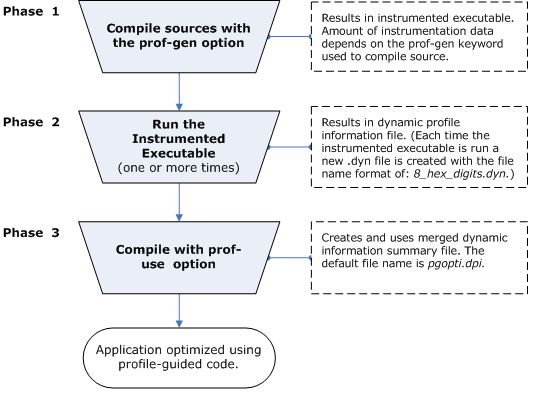
\includegraphics[width=0.75\textwidth]{images/pogo-workflow.jpg}
\end{center}

\end{frame}



\begin{frame}
\frametitle{Save Some Steps}



Not necessary to do all three steps for every build. 

Re-use training data while it's still valid.

Recommended dev workflow:
\begin{itemize}
\item dev A performs these steps, checks the training data into source control
\item whole team can use profiling information for their compiles.
\end{itemize}


\end{frame}



\begin{frame}
\frametitle{Not fixing all the problems in the world}



What does it mean for it to be better? 

The algorithms will aim for speed in areas that are ``hot''. 

The algorithms will aim for minimal code size in areas that are ``cold'' .

Less than 5\% of methods compiled for speed.

\end{frame}



\begin{frame}
\frametitle{Combining Training Runs}



Can combine multiple training runs and manually give suggestions about important scenarios.

The more a scenario runs in the training data, \\
the more important it will be, from POGO's point of view.

Can merge multiple runs with user-assigned weightings.


\end{frame}


\begin{frame}[fragile]
\frametitle{Full Test Scenario}

{\scriptsize
\begin{verbatim}
# STEP 1: Compile the binary with instrumentation
rustc -Cprofile-generate=/tmp/pgo-data -O ./main.rs

# STEP 2: Run the binary a few times, maybe with common sets of args.
#         Each run will create or update `.profraw` files in /tmp/pgo-data
./main mydata1.csv
./main mydata2.csv
./main mydata3.csv

# STEP 3: Merge and post-process all the `.profraw` files in /tmp/pgo-data
llvm-profdata merge -o ./merged.profdata /tmp/pgo-data

# STEP 4: Use the merged `.profdata` file during optimization. All `rustc`
#         flags have to be the same.
rustc -Cprofile-use=./merged.profdata -O ./main.rs
\end{verbatim}
}

\end{frame}



\begin{frame}
\frametitle{Behind the Scenes}



In the optimize phase, compiler uses the training data for:

\begin{enumerate}
\item Full and partial inlining
\item Function layout
\item Speed and size decision
\item Basic block layout 
\item Code separation
\item Virtual call speculation
\item Switch expansion
\item Data separation
\item Loop unrolling
\end{enumerate}

\end{frame}



\begin{frame}
\frametitle{Muh Gainz}



Most performance gains from inlining.

Decisions based on the call graph path profiling. 

But: behaviour of function \texttt{foo} may be very different when called from \texttt{B} than when called from \texttt{D}. 


\begin{center}
	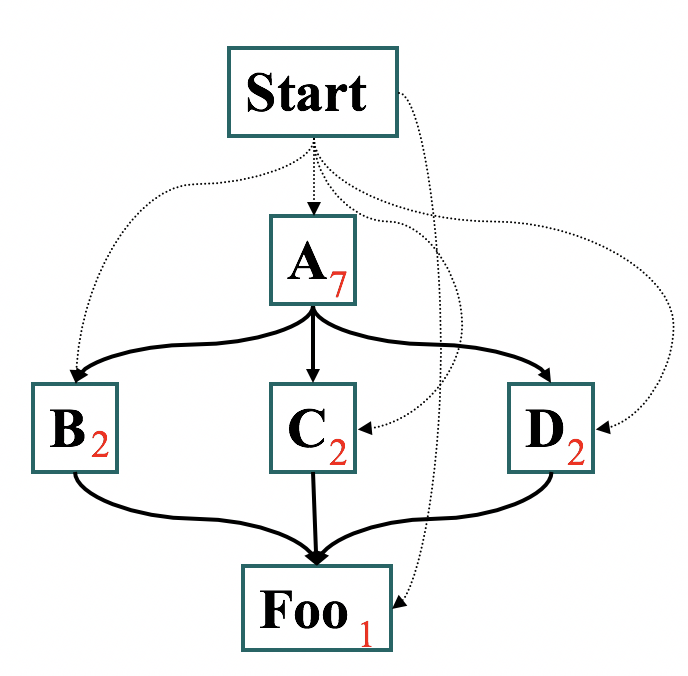
\includegraphics[width=0.4\textwidth]{images/callpaths.png}
\end{center}

\end{frame}



\begin{frame}
\frametitle{Another Call Graph}


Example 2 of relationships between functions.\\
Numbers on edges represent the number of invocations:

\begin{center}
	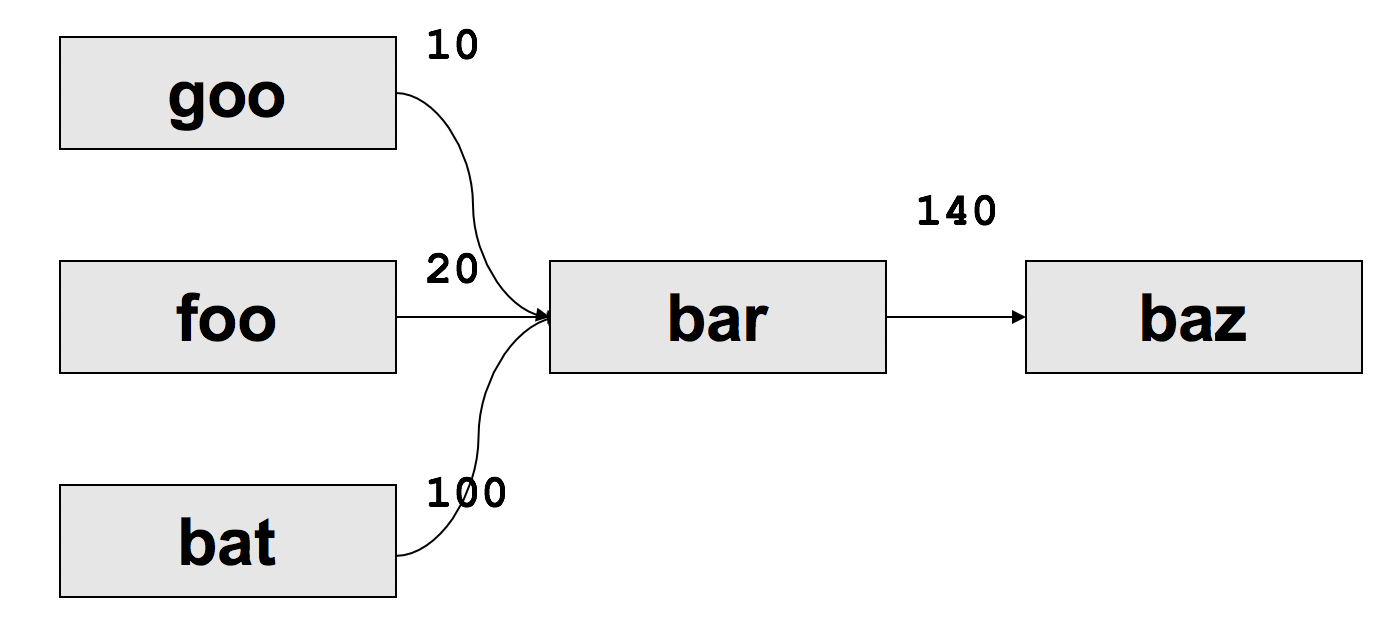
\includegraphics[width=\textwidth]{images/callpaths2.png}
\end{center}

\end{frame}



\begin{frame}
\frametitle{The POGO View of the World}

When considering what to do here, POGO takes the view like this:

\begin{center}
	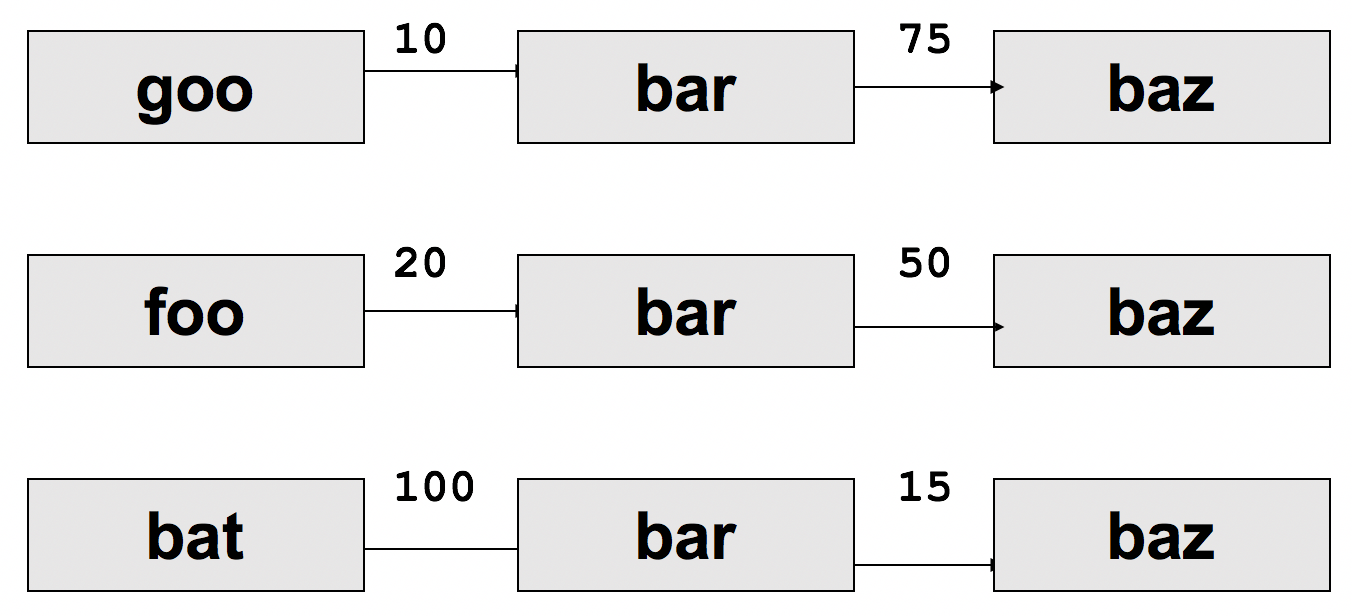
\includegraphics[width=\textwidth]{images/callpaths3.png}
\end{center}

\end{frame}



\begin{frame}
\frametitle{The POGO View of the World}

\begin{center}
	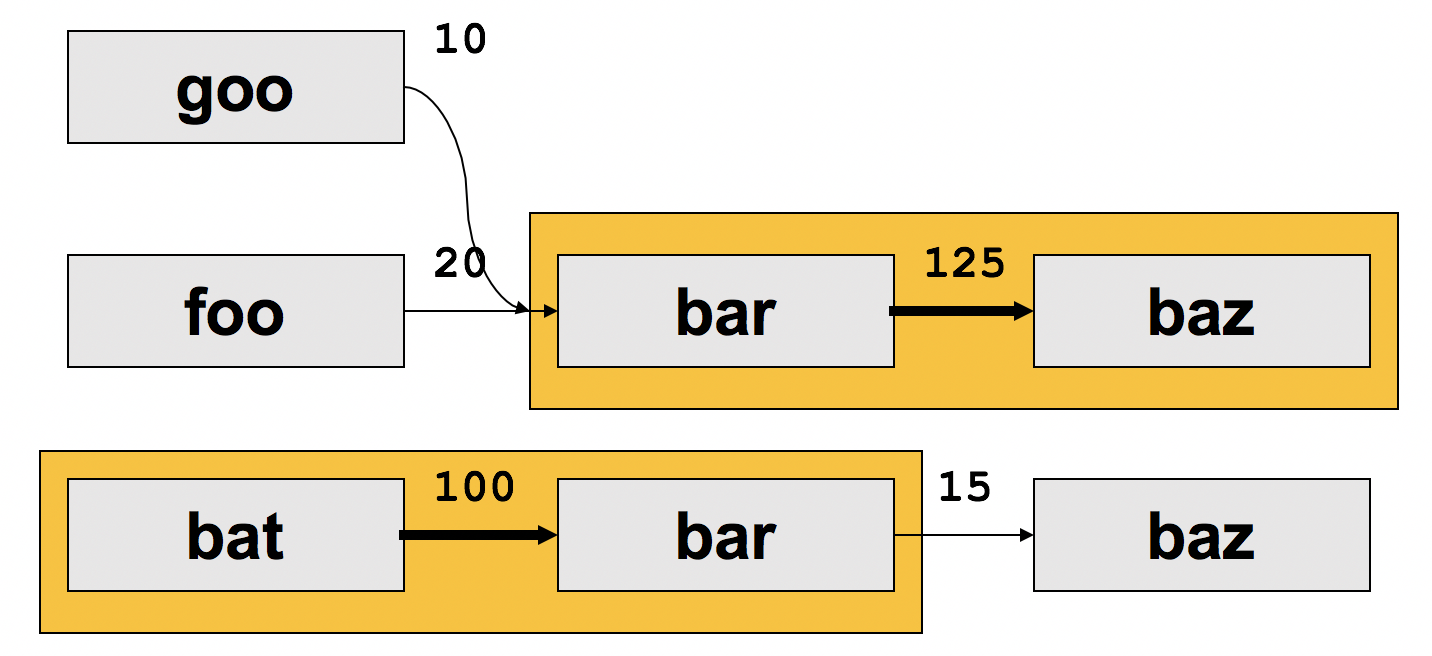
\includegraphics[width=\textwidth]{images/callpaths4.png}
\end{center}

\end{frame}




\begin{frame}
\frametitle{Page Locality}



Call graph profiling data also good for packing blocks.

Put most common cases nearby.\\
Put successors after their predecessors.

Packing related code = fewer page faults (cache misses).

Calling a function in same page as caller =  ``page locality''.


\end{frame}



\begin{frame}
\frametitle{Block Layout}

\begin{center}
	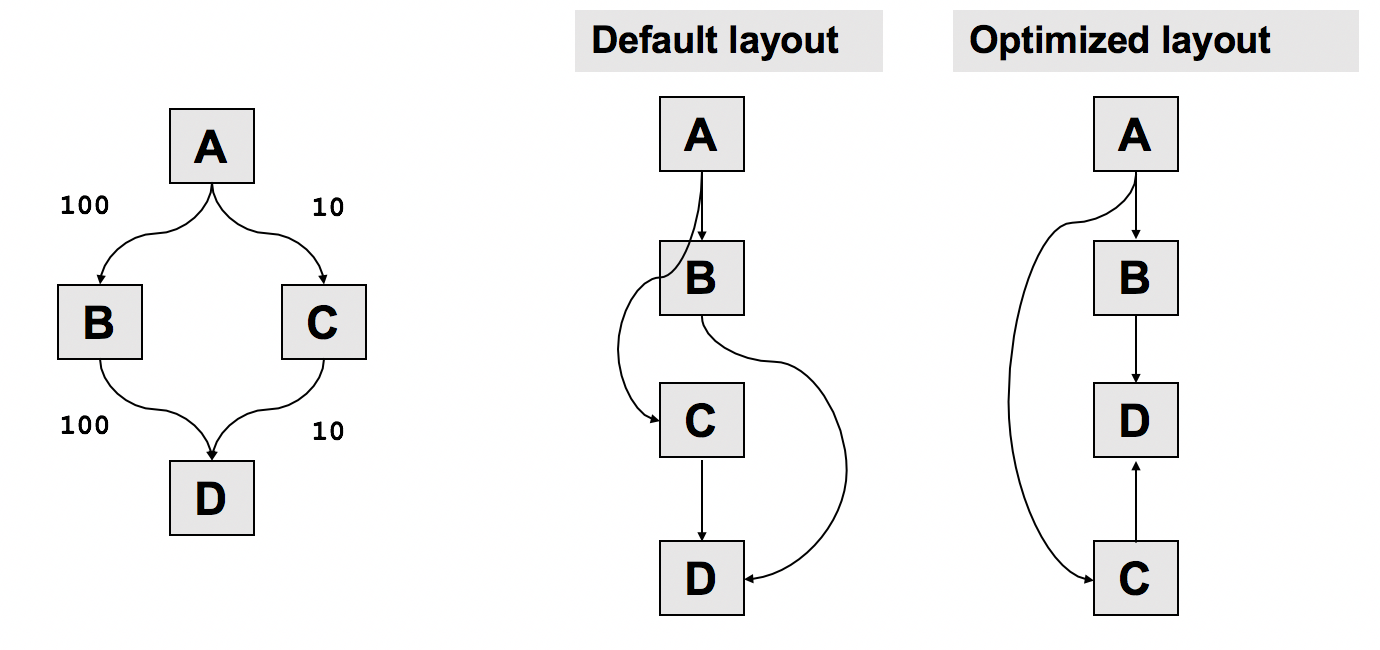
\includegraphics[width=\textwidth]{images/blocklayout.png}
\end{center}

\end{frame}



\begin{frame}
\frametitle{Dead Code?}



According to the author, ``dead'' code goes in its own special block. 

Probably not truly dead code (compile-time unreachable).

Instead: code that never gets invoked in training.


\end{frame}



\begin{frame}
\frametitle{Benchmark Results}
 
OK, how well does POGO work?

The application under test is a standard benchmark suite (Spec2K):


\begin{center}
\begin{tabular}{l|l|l|l|l|l}
	\textbf{Spec2k:} & \textbf{sjeng} & \textbf{gobmk} & \textbf{perl} & \textbf{povray} & \textbf{gcc}\\ \hline
	\textbf{App Size:} &  {Small} & {Medium} & {Medium} & {Medium} & {Large} \\ \hline
	\textbf{Inlined Edge Count} & 50\% & 53\% & 25\% & 79\% & 65\% \\ \hline
	\textbf{Page Locality} & 97\% & 75\% & 85\% & 98\% & 80\% \\ \hline
	\textbf{Speed Gain} & 8.5\% & 6.6\% & 14.9\% & 36.9\% & 7.9\% \\ 
\end{tabular}
\end{center}

 
We can speculate about how well synthetic benchmarks results translate to real-world application performance\ldots


\end{frame}



\end{document}

